\documentclass[border=5pt]{standalone}
\usepackage{tikz}
\usepackage{amsmath}
\usetikzlibrary{calc, positioning, arrows.meta}
\begin{document}
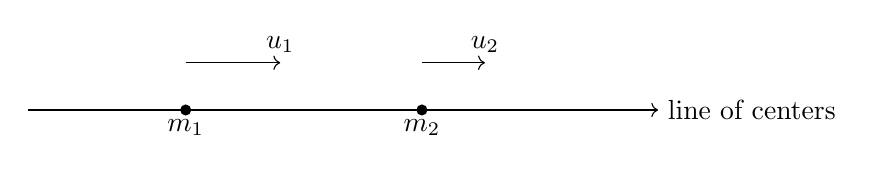
\begin{tikzpicture}[scale=1.0]
  % pre-collision velocities
  \draw[->] (-4,0) -- (4,0) node[right] {line of centers};
  \fill (-2,0) circle (2pt) node[below] {$m_1$};
  \fill (1,0) circle (2pt) node[below] {$m_2$};
  \draw[->] (-2,0.6) -- (-0.8,0.6) node[above] {$u_1$};
  \draw[->] (1,0.6) -- (1.8,0.6) node[above] {$u_2$};
\end{tikzpicture}
\end{document}
